\documentclass[unnumsec,webpdf,contemporary,large]{oup-authoring-template}

\graphicspath{{Fig/}}

\theoremstyle{thmstyleone}
\newtheorem{theorem}{Theorem}
\newtheorem{proposition}[theorem]{Proposition}
\theoremstyle{thmstyletwo}
\newtheorem{example}{Example}
\newtheorem{remark}{Remark}
\theoremstyle{thmstylethree}
\newtheorem{definition}{Definition}

\begin{document}

\journaltitle{CS6024}
\copyrightyear{2026}
\pubyear{2026}
\appnotes{Research Project}

\firstpage{1}

\title[Stress testing PCA]{An evaluation of PCA for detecting population stratification in admixed populations}

\author[]{Krutarth Patel}

\address[]{\orgdiv{EE23B137}}

\abstract{
    \textit{Motivation:} PCA is an industry standard tool for removing population stratification in GWAS studies. While the algorithm is well understood, the interpretation of the output is debatable. \textit{Results:} Here, we evaluate PCA in various synthesized scenarios to test the robustness and validity of PCA. We identify the failure modes of PCA that either result in loss of power or false associations in GWAS studies. \textit{Availability and Implementation:} A framework for testing PCA using various sources of synthesized data is available freely at \url{https://github.com/kuku929/pca-gwas}.
}

\keywords[GWAS]{Genome Wide Association Study}
\keywords[PCA]{Principal Component Analysis}

\maketitle

\section{Introduction}
GWAS studies associate trait variation with genetic loci. In the past, GWAS studies have successfully identified genetic causes of diseases and other phenotypes(reference). However, GWAS studies can be confounded by many factors not limited to environmental confounding, population stratification, cryptic relatedness. Population stratification is a false association of ancestry-based genetic differences to traits of interest in a study. Accounting for population stratification has become increasingly crucial as GWAS studies have scaled to include millions(? reference) of individuals. Population structure in GWAS cohorts takes three forms \citep{Li2010}. \textit{Discrete} structure arises when genetically divergent populations are studied together, such as Europeans, Africans, and Asians; individuals cluster cleanly and separation is straightforward. \textit{Admixed} structure occurs when individuals carry ancestry from multiple source populations in varying proportions — as seen in African Americans and Hispanic Americans — precluding clean cluster assignment. \textit{Hierarchical} structure combines both: discrete subpopulations each containing admixed individuals, increasingly common in large multi-ethnic consortia.
Modern studies use various tools to remove these confounding factors before making any associations between SNPs and traits. Some popular tools for removing population stratification are: PLINKv2.0(reference), Bolt LMM(reference), ADMIXTURE(reference), STRUCTURE(reference).

Most studies use PCA as a step in their pipeline for removing stratification. In this study we evaluate PLINKv2.0's PCA implementation against synthesized data obtained from HAPNEST(reference) and msprime(reference) to identify cases where PCA fails to reduce stratification to an acceptable level.

Using HAPNEST, we generate synthetic genotypes and construct five cohorts: a continuous EUR to AFR admixture gradient, a three-way admixture triangle (EUR, AFR, EAS), an admixed-majority cohort where admixed individuals outnumber ancestral populations, a sweep over admixed fraction from 0\% to 100\%, and a differential heritability experiment where source populations carry different $h^2$ values. Using msprime \citep{msprime}, we construct four cases: an admixture timing sweep varying the number of generations since the admixture event, a ghost population experiment where one ancestry source is absent from the cohort, an isolation-by-distance stepping-stone model with 16 populations along a geographic gradient, and a comparison of pulse versus continuous gene flow. Across all experiments, stratification correction is quantified via the genomic inflation factor $\lambda$, measured at 0, 2, 5, 10, and 20 principal components.

\section{Materials and Methods}

\subsection{Datasets and Preprocessing}
We use two synthetic data generators to produce hypothetical cohorts.

\subsubsection{HAPNEST}
We generate synthetic genotypes and phenotypes using the 1000 Genomes and HGDP reference panels \citep{hapnest}. All experiments use only chromosome 2 data with MAF $\geq 1\%$, yielding 111,760 SNPs. All tests use a polygenicity of 0.005 ($\approx 559$ causal SNPs). The same causal SNPs act across all populations (pleiotropy $= 1.0$). All experiments have a fixed heritability $h^2 = 0.1$ except in the differential heritability experiment where $h^2_{\text{EUR}} = 0.3$ and $h^2_{\text{AFR}} = 0.01$. No environmental covariates affect the observed phenotype. With these assumptions, any inflation in the genomic inflation factor can be attributed entirely to population stratification.

\subsubsection{msprime}
All simulations use a 10\,Mb sequence, recombination rate $r = 10^{-8}$ per bp per generation, and mutation rate $\mu = 1.29 \times 10^{-8}$ per bp per generation under the JC69 model \citep{msprime}, yielding approximately 48,000--370,000 segregating sites before filtering. After applying a MAF $\geq 1\%$ filter, multiallelic sites are excluded. Phenotypes are assigned as a linear function of population ancestry label rather than genotype:
\begin{equation}
    Y_i = \alpha \cdot s_i + \sqrt{1 - \alpha^2}\,\varepsilon_i, \quad \varepsilon_i \sim \mathcal{N}(0,1)
\end{equation}
where $s_i$ is a population-specific ancestry score (standardised to zero mean, unit variance) and $\alpha = 0.8$ controls confounding strength. This ensures all observed inflation is attributable to stratification, with no true genetic signal.

\subsection{Algorithms}
We consider two algorithms for comparison.

\subsubsection{PLINKv2.0}
PCA calculates a low-dimensional approximation of the genotype matrix ($\#\text{SNPs} \times \#\text{individuals}$). The resultant matrix is a projection of individuals onto the plane of maximum variance. The biggest source of variance among individuals is their ancestry. Thus the projected data quantifies the ancestry of individuals.

Association testing was performed using PLINKv2.0 \citep{plink2} with the linear regression model (\texttt{--glm hide-covar}). A MAF filter of $\geq 1\%$ was applied at the association step. Principal components were computed from the genotype matrix using PLINKv2.0's \texttt{--pca} implementation, which performs an eigendecomposition of the standardised genotype matrix. For each SNP, plink2 fits:
$$Y_i = \beta_0 + \beta_{\text{SNP}} X_i + \sum_{j=1}^{k} \gamma_j \text{PC}_{ij} + \varepsilon_i$$
where $Y_i$ is the phenotype of individual $i$, $X_i$ is the allele count at that SNP, and $\text{PC}_{ij}$ is the $j^{\text{th}}$ principal component score of individual $i$.

\subsubsection{BOLT-LMM}
BOLT-LMM \citep{boltlmm} models population structure implicitly via a linear mixed model. Rather than including explicit PC covariates, it fits a random effect whose covariance structure is defined by the genetic relationship matrix (GRM), computed directly from the genotype data. The model is:
\begin{equation}
    \mathbf{y} = \mathbf{x}\beta + \mathbf{g} + \boldsymbol{\varepsilon}, \quad
    \mathbf{g} \sim \mathcal{N}(\mathbf{0},\, \sigma^2_g \mathbf{K}), \quad
    \boldsymbol{\varepsilon} \sim \mathcal{N}(\mathbf{0},\, \sigma^2_e \mathbf{I})
\end{equation}
where $\mathbf{x}$ is the SNP genotype vector, $\beta$ is the fixed effect of interest, $\mathbf{g}$ is the polygenic random effect, and $\mathbf{K}$ is the GRM.

BOLT-LMM was run with \texttt{--lmmForceNonInf} to use the full non-infinitesimal LMM rather than the faster infinitesimal approximation, and \texttt{--LDscoresUseChip} to compute LD scores from the input genotypes. P-values were taken from the \texttt{P\_BOLT\_LMM} column of the output and $\lambda$ computed identically to the PCA-based analysis.

\subsection{Genomic Inflation Factor ($\lambda$)}
\citet{Devlin1999} provided a statistic (denoted by $\lambda$) which can be used to measure population stratification in a cohort. For each SNP under the null hypothesis (no association) the GWAS statistic follows a $\chi^2$ distribution. The expected median of this distribution is $0.456$. If there is population stratification in the samples, the expected median will be $> 0.456$ due to false positives. Thus, we define $\lambda$ as:
\begin{equation}
    \lambda = \frac{\text{median}(\chi^2_{\text{obs}})}{0.456}
\end{equation}

\subsection{HAPNEST Experiments}
Five cohort designs were evaluated:

\begin{enumerate}
\item \textbf{Admixture gradient.} Five groups spanning a EUR--AFR ancestry spectrum: pure EUR ($n=200$), 75\% EUR ($n=100$), 50\% EUR ($n=100$), 25\% EUR ($n=100$), and pure AFR ($n=200$). Total $N=700$.

\item \textbf{Three-way admixture.} Seven groups forming a triangle over EUR, AFR, and EAS ancestry: three pure-ancestry anchors ($n=150$ each), three pairwise admixed groups ($n=100$ each), and one three-way admixed group ($n=100$). Total $N=850$.

\item \textbf{Admixed-majority overwhelm.} A severely unbalanced cohort of pure EUR ($n=30$), pure AFR ($n=30$), and 50\% EUR/AFR admixed individuals ($n=500$). The admixed majority dominates the variance structure seen by PCA. Total $N=560$.

\item \textbf{Admixture sweep.} Five independent GWAS runs sweeping the admixed fraction from 0\% to 100\% in 25\% increments, holding total $N=700$ constant. This isolates the effect of admixed fraction on inflation.

\item \textbf{Differential heritability.} A two-population cohort (EUR $n=350$, AFR $n=350$) with population-specific heritabilities ($h^2_{\text{EUR}}=0.3$, $h^2_{\text{AFR}}=0.01$), isolating the effect of genetic architecture heterogeneity.
\end{enumerate}

\subsection{msprime Experiments}
Four experiments were conducted:

\begin{enumerate}
\item \textbf{Admixture timing sweep.} A fixed EUR--AFR admixed cohort (EUR $n=200$, AFR $n=200$, ADMIX $n=300$, 50/50 proportions) was simulated at seven admixture times $T \in \{2, 5, 10, 20, 50, 100, 200\}$ generations ago, holding all other parameters constant. Ancestry scores: EUR $= 1$, AFR $= 0$, ADMIX $= 0.5$. This tests whether the recency of admixture affects PCA's ability to resolve ancestry axes.

\item \textbf{Ghost population.} Three populations A, C, and ADMIX$_{\text{AC}}$ (50\% A $+$ 50\% C, admixed $T=50$ generations ago) were simulated, with A and C diverging from a common ancestor at $T=1000$ generations. The GWAS cohort contains only A ($n=400$) and ADMIX$_{\text{AC}}$ ($n=300$); population C is never sampled.

\item \textbf{Ghost C-sample sweep.} To quantify the effect of introducing pure C reference samples, the base cohort (A $n=400$, ADMIX$_{\text{AC}}$ $n=300$) was held fixed while sweeping the number of added C samples over $n_C \in \{0, 25, 50, 100, 200, 400\}$.

\item \textbf{Isolation by distance.} A 1D stepping-stone model with $K=16$ populations of equal size ($N_e = 10{,}000$) connected by nearest-neighbour migration at rate $m = 10^{-3}$ per generation was simulated \citep{Novembre2008}. Phenotype score is proportional to geographic position (population index / $(K-1)$). Two sampling strategies were compared: (a) uniform sampling across all 16 populations ($n=44$ per population, total $N=704$), and (b) sampling only the two endpoint populations ($n=350$ each, total $N=700$).

\item \textbf{Pulse versus continuous gene flow.} Two scenarios with the same mean admixture proportion were compared. In the pulse scenario, a single admixture event at $T=50$ generations introduced EUR ancestry at 50\% proportion (EUR $n=200$, AFR $n=200$, ADMIX $n=300$). In the continuous scenario, symmetric migration between EUR and AFR at rate $m=0.02$ per generation operated for 50 generations (EUR $n=350$, AFR $n=350$).
\end{enumerate}

\section{Progress after Intermediate Results}

The HAPNEST experiments established that PCA performs adequately under standard admixture scenarios but shows consistent residual inflation under intermediate admixture fractions and differential heritability. These results, while informative, reflect realistic but relatively mild failure modes — $\lambda$ values in the range 1.01--1.03, close to the commonly accepted threshold of 1.05. To probe more fundamental limitations of PCA, we turned to msprime to construct scenarios with known theoretical failure modes where inflation is expected to persist regardless of the number of PCs included.

msprime allows precise control over demographic history — admixture timing, migration rates, population topology, and sample composition — which HAPNEST, being tied to the 1000 Genomes and HGDP reference panels, cannot provide. This makes it possible to isolate individual failure conditions cleanly and test theoretical predictions directly.

\section{Results and Discussion}

\subsection{HAPNEST Experiments}

Table~\ref{tab:hapnest} summarises $\lambda$ across all HAPNEST experiments at $k \in \{2, 5, 10\}$ PC covariates alongside BOLT-LMM. We find that PCA performs well in most structured scenarios but breaks down under differential heritability, and that BOLT-LMM does not consistently outperform PCA.

\begin{table}[!t]
\caption{Genomic inflation factor $\lambda$ for HAPNEST experiments. Lower values indicate better correction.\label{tab:hapnest}}
\begin{tabular*}{\columnwidth}{@{\extracolsep\fill}lcccc@{\extracolsep\fill}}
\toprule
Experiment & PC2 & PC5 & PC10 & BOLT-LMM \\
\midrule
Admixture gradient         & 1.007 & 0.999 & 1.002 & 1.251 \\
Three-way admixture        & 0.994 & 1.000 & 0.995 & 0.998 \\
Admixed majority overwhelm & 0.977 & 0.979 & 0.981 & 0.998 \\
Differential heritability  & 1.007 & 1.010 & 1.013 & 0.865 \\
Admixture sweep 25\%       & —     & —     & 1.020 & 1.094 \\
Admixture sweep 50\%       & —     & —     & 1.008 & 1.045 \\
Admixture sweep 75\%       & —     & —     & 1.026 & 1.045 \\
Admixture sweep 100\%      & —     & —     & 0.989 & 0.998 \\
\botrule
\end{tabular*}
\end{table}

\begin{figure}[!t]
\centering
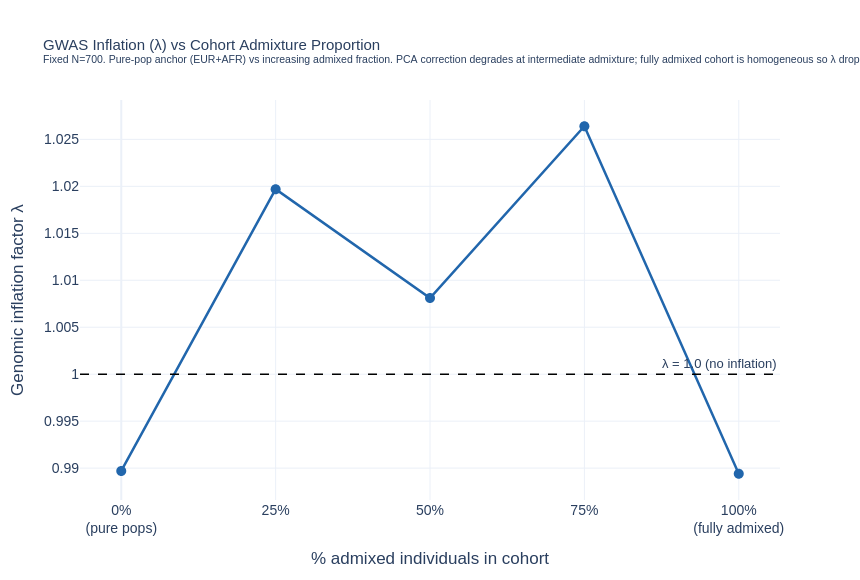
\includegraphics[width=0.48\textwidth]{sweep.png}
\caption{Effect of admixed fraction on $\lambda$ at PC10.\label{fig:sweep}}
\end{figure}

The admixture gradient reaches $\lambda \approx 1.00$ with just 2 PCs. This is the scenario PCA is designed for — PC1 aligns with the EUR--AFR allele frequency axis and conditioning on it removes the dominant confound. BOLT-LMM performs noticeably worse here ($\lambda = 1.251$), likely because the GRM treats admixed intermediate individuals as partially related to both ancestry groups, inflating rather than correcting the test statistics. The three-way admixture and admixed majority experiments are similarly well-corrected by PCA at PC10.

The admixture sweep (Figure~\ref{fig:sweep}) shows a non-monotonic pattern: $\lambda$ peaks at 25\% and 75\% admixed and returns to $\approx 1.00$ at 0\% and 100\%. At intermediate admixture fractions, the cohort contains both discrete and admixed individuals simultaneously, and PCA axes cannot cleanly separate all ancestry components. A fully admixed cohort is essentially homogeneous from PCA's perspective and stratification disappears.

The differential heritability experiment is the most revealing HAPNEST result. Even though PC1 cleanly separates EUR from AFR, inflation persists and slightly worsens with more PCs ($\lambda_{\text{PC10}} = 1.013$). This shows that PCA corrects mean allele-frequency differences between populations but cannot correct heterogeneity in causal effect sizes. When $h^2_{\text{EUR}} = 0.3$ and $h^2_{\text{AFR}} = 0.01$, EUR-enriched causal variants drive associations that no ancestry covariate can remove. Interestingly, BOLT-LMM over-corrects here ($\lambda = 0.865$).

\subsection{msprime Experiments}

\subsubsection{Admixture Timing}

Table~\ref{tab:timing} shows $\lambda$ across admixture times $T$ and Figure~\ref{fig:timing} plots these results. The uncorrected $\lambda$ at $k=0$ is uniformly around 24 across all $T$ values, confirming that the phenotype-ancestry confound is present in every scenario. After correction, $T=10$ generations is the hardest case — $\lambda$ remains at 1.063 even at PC20. Very recent admixture ($T=2$) and ancient admixture ($T \geq 100$) are both well corrected. At $T=2$, ancestry tracts span large genomic blocks and produce a strong, coherent PC signal. At $T \geq 100$, extensive recombination has broken down ancestry tracts and populations approach panmixia. At $T \approx 10$, tracts are fragmented enough to produce heterogeneous ancestry across individuals but structured enough to confound GWAS — this is the intermediate regime where PCA struggles most.

\begin{figure}[!t]
\centering
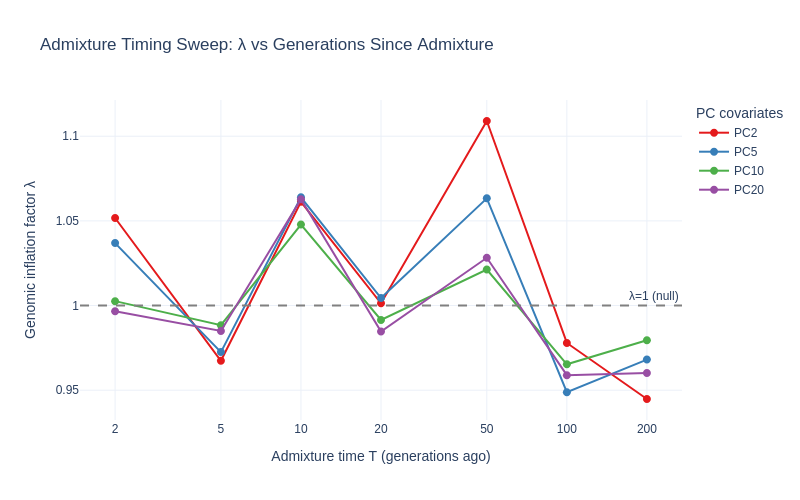
\includegraphics[width=0.48\textwidth]{timing_lambda.png}
\caption{Admixture timing sweep: $\lambda$ vs generations since admixture (log scale).\label{fig:timing}}
\end{figure}

\begin{table}[!t]
\caption{Admixture timing sweep: $\lambda$ at varying PC counts. $T$ = generations since admixture.\label{tab:timing}}
\begin{tabular*}{\columnwidth}{@{\extracolsep\fill}rcccc@{\extracolsep\fill}}
\toprule
$T$ (gens) & PC2 & PC5 & PC10 & PC20 \\
\midrule
2   & 1.052 & 1.037 & 1.003 & 0.997 \\
5   & 0.967 & 0.973 & 0.988 & 0.985 \\
10  & 1.061 & 1.064 & 1.048 & 1.063 \\
20  & 1.001 & 1.004 & 0.992 & 0.985 \\
50  & 1.109 & 1.063 & 1.021 & 1.028 \\
100 & 0.978 & 0.949 & 0.965 & 0.959 \\
200 & 0.945 & 0.968 & 0.980 & 0.960 \\
\botrule
\end{tabular*}
\end{table}

\subsubsection{Ghost Population}

Figure~\ref{fig:ghost} shows the ghost population result. When population C is absent from the cohort, $\lambda$ plateaus at $\approx 1.12$ and stays flat across all PC counts. When C is added as a control ($n=150$), $\lambda$ starts higher ($1.49$ at PC2) but decreases with more PCs, confirming that PCA can correct the inflation once the ancestry axis is visible. This shows that PCA cannot fully account for stratification due to populations present in admixed individuals only.

\begin{figure}[!t]
\centering
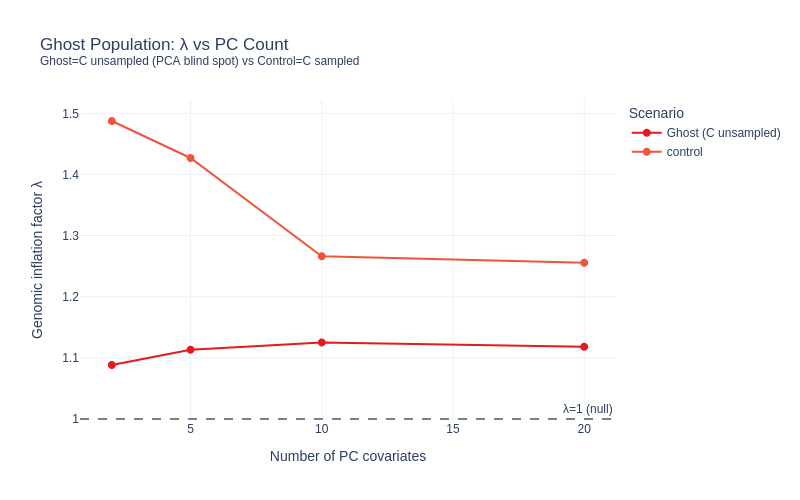
\includegraphics[width=0.48\textwidth]{ghost_lambda.png}
\caption{Ghost population: $\lambda$ vs PC count. Ghost = C unsampled; Control = C sampled.\label{fig:ghost}}
\end{figure}

Figure~\ref{fig:csweep} shows what happens as we vary the number of C samples added to the base cohort. Adding C samples does not help and in fact increases $\lambda$ monotonically. With zero C samples, $\lambda \approx 1.09$--$1.13$; adding 400 C samples raises this to $1.23$--$1.61$. Introducing C creates a new stratification axis that PCA detects, but since admixed individuals are intermediate on this axis, correction is not effective enough. This has a practical implication: adding reference individuals from an unsampled ancestry source to a GWAS cohort does not guarantee better stratification correction.

\begin{figure}[!t]
\centering
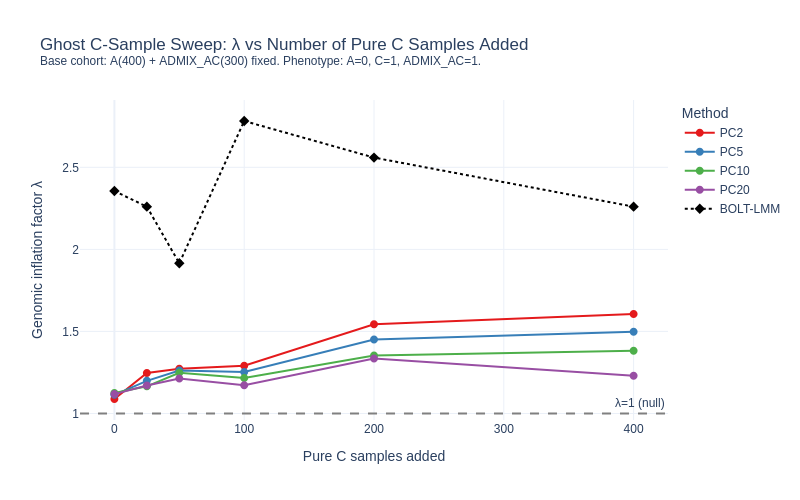
\includegraphics[width=0.48\textwidth]{ghost_c_sweep.png}
\caption{Ghost C-sample sweep: $\lambda$ vs number of pure C samples added to base cohort (A $n=400$, ADMIX$_{\text{AC}}$ $n=300$).\label{fig:csweep}}
\end{figure}

\subsubsection{Isolation by Distance}

Table~\ref{tab:stepping} shows results for the stepping-stone model. With all 16 populations sampled, $\lambda$ decreases slowly from $1.70$ at PC2 to $1.04$ at PC20 — still above 1 even with 20 PCs. The confounding here is due to a continuous geographic gradient. The endpoints-only scenario is more practically relevant: sampling only the two geographically extreme populations gives $\lambda \approx 1.07$ regardless of PC count. A researcher in this situation would see two apparently discrete populations and expect 1--2 PCs to suffice, but the shared clinal ancestry history inflates test statistics in a way that a simple two-population PCA cannot resolve.

\begin{table}[!t]
\caption{Stepping-stone model: $\lambda$ for full gradient vs endpoints-only sampling.\label{tab:stepping}}
\begin{tabular*}{\columnwidth}{@{\extracolsep\fill}lcccc@{\extracolsep\fill}}
\toprule
Scenario & PC2 & PC5 & PC10 & PC20 \\
\midrule
Full gradient (16 pops) & 1.696 & 1.259 & 1.094 & 1.041 \\
Endpoints only (2 pops) & 1.081 & 1.072 & 1.101 & 1.069 \\
\botrule
\end{tabular*}
\end{table}

\subsubsection{Pulse versus Continuous Gene Flow}

Table~\ref{tab:flow} compares pulse and continuous gene flow. The pulse scenario reaches $\lambda \approx 1.02$ at PC10, consistent with standard admixture results. The continuous flow scenario behaves differently: $\lambda \approx 1.13$--$1.17$ across all PC counts with no sign of convergence. Continuous migration creates a distribution of ancestry proportions within each labelled population rather than a fixed proportion. PCA captures the mean EUR--AFR difference but cannot resolve the variance around it, so each additional PC fails to reduce inflation further.

\begin{table}[!t]
\caption{Pulse vs continuous gene flow: $\lambda$ at varying PC counts.\label{tab:flow}}
\begin{tabular*}{\columnwidth}{@{\extracolsep\fill}lcccc@{\extracolsep\fill}}
\toprule
Scenario & PC2 & PC5 & PC10 & PC20 \\
\midrule
Pulse admixture & 1.109 & 1.063 & 1.021 & 1.028 \\
Continuous flow & 1.173 & 1.150 & 1.132 & 1.172 \\
\botrule
\end{tabular*}
\end{table}

\subsection{Discussion}

Across all experiments, PCA works well for the scenario it was designed for — discrete, well-separated populations — but we identify three conditions where it fails. First, intermediate admixture timing ($T \approx 10$ generations) produces fragmented ancestry that resists correction. Second, absent ancestry sources make PCA correction incomplete regardless of the number of PCs. Third, genetic architecture heterogeneity is a failure mode that PCA cannot address by design.

BOLT-LMM does not consistently outperform PCA. It performs better in some discrete population scenarios but worse under admixture, particularly in the ghost population and continuous flow experiments.

\section{Conclusion}

In this study we evaluated PCA-based stratification correction across nine HAPNEST experiments and four msprime simulations, measuring $\lambda$ at 0, 2, 5, 10, and 20 principal components. We find that PCA performs well in the scenarios it was designed for but fails predictably under four conditions: intermediate admixture timing ($T \approx 10$ generations), ghost populations where ancestry sources are absent from the cohort, continuous gene flow creating within-group ancestry variance, and genetic architecture heterogeneity across populations.

BOLT-LMM does not consistently outperform PCA. It performs better in some discrete population scenarios but worse under admixture, particularly when ancestry sources are unsampled or when within-group ancestry variance is high.

\section{Future Work}

The ghost population result suggests that the reference panels used to supplement GWAS cohorts matters significantly — adding ancestry representatives that are not present in the study population can worsen stratification rather than improve it. A criterion for when adding a reference panel helps versus hurts would be practically valuable.

The admixture timing result motivates a closer investigation of recent admixture in biobank-scale cohorts. As biobanks increasingly include recently admixed populations, the $T \approx 10$ regime will become more common and standard PC-based pipelines may underperform. Finally, none of the methods tested here — PCA or BOLT-LMM — adequately handle continuous gene flow. Methods that explicitly model ancestry as a continuous distribution rather than a discrete assignment may be better suited to these scenarios.

\section*{Data Availability}
All code is available at \url{https://github.com/kuku929/pca-gwas}.

\bibliographystyle{oup-abbrvnat}
\bibliography{reference}

\begin{appendices}

\section{Additional Figures}

\begin{figure}[!h]
\centering
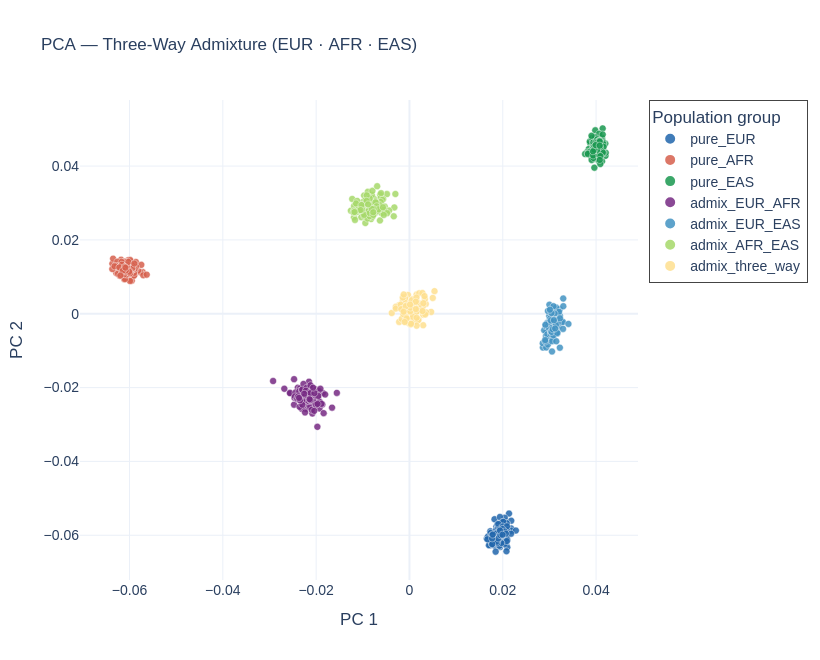
\includegraphics[width=0.48\textwidth]{three_way.png}
\caption{Three-way admixture (EUR, AFR, EAS): $\lambda$ vs PC count.\label{fig:three_way}}
\end{figure}

\begin{figure}[!h]
\centering
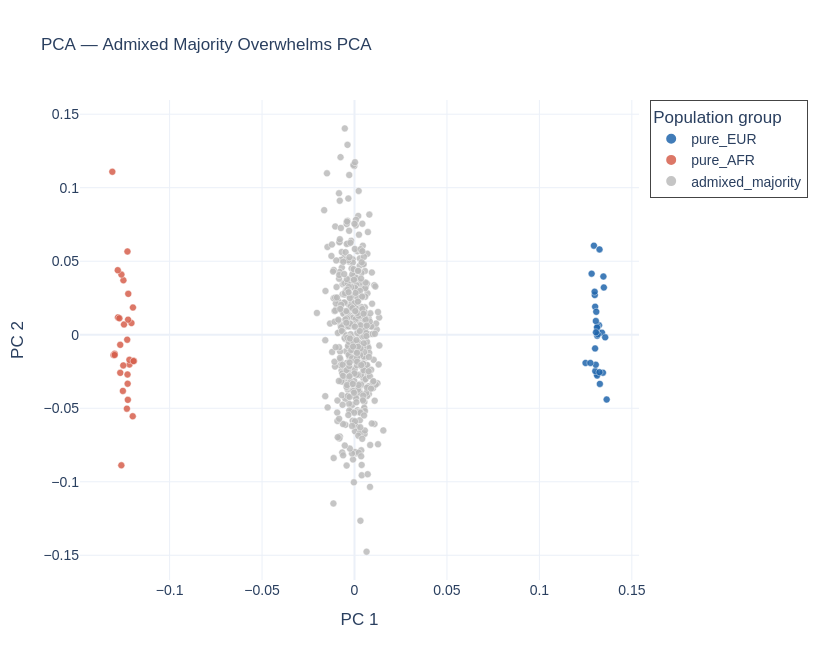
\includegraphics[width=0.48\textwidth]{maj_admix.png}
\caption{Admixed majority overwhelm: $\lambda$ vs PC count.\label{fig:maj_admix}}
\end{figure}

\begin{figure}[!h]
\centering
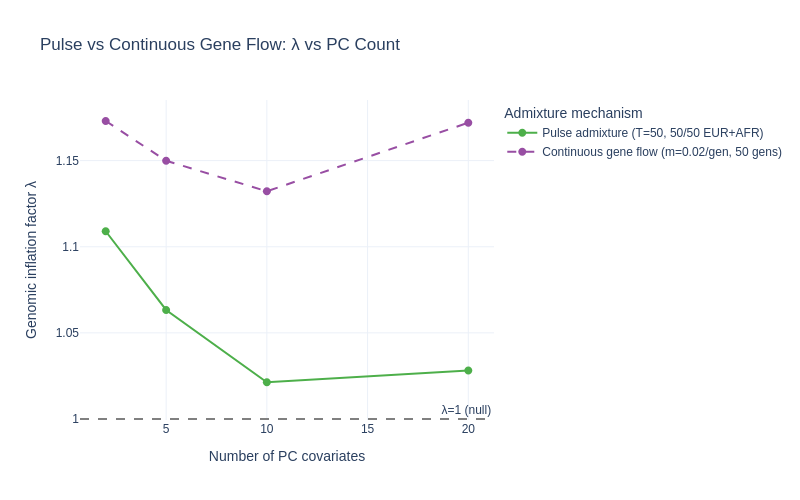
\includegraphics[width=0.48\textwidth]{pulse.png}
\caption{Pulse vs continuous gene flow: $\lambda$ vs PC count.\label{fig:pulse}}
\end{figure}

\begin{figure}[!h]
\centering
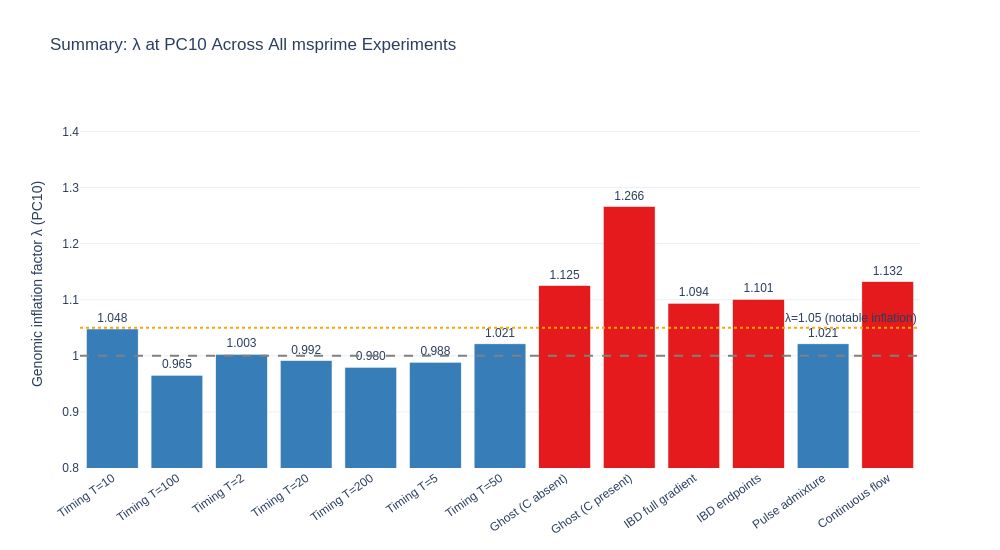
\includegraphics[width=0.48\textwidth]{summary.png}
\caption{Summary: $\lambda$ at PC10 across all msprime experiments.\label{fig:summary}}
\end{figure}

\end{appendices}

\end{document}
